\documentclass[12pt, openany]{report}
\usepackage[utf8]{inputenc}
\usepackage[T1]{fontenc}
\usepackage[a4paper,left=2cm,right=2cm,top=2cm,bottom=2cm]{geometry}
%\usepackage{natbib}
\usepackage[french]{babel}
\usepackage{libertine}
\usepackage[pdftex]{graphicx}
\usepackage{lipsum}
\usepackage[colorlinks = true,
            linkcolor = black,
            urlcolor  = blue]{hyperref}

%\setlength{\parindent}{0cm}
\setlength{\parskip}{1ex plus 0.5ex minus 0.2ex}
\newcommand{\hsp}{\hspace{20pt}}
\newcommand{\HRule}{\rule{\linewidth}{0.5mm}}

\begin{document}

\begin{titlepage}
  \begin{rmfamily}
  \begin{center}

    % Upper part of the page. The '~' is needed because \\
    % only works if a paragraph has started.
    ~\\[2cm]

    \textsc{\LARGE Universit\'e Polytechnique Hauts-de-France}~\\[0.5cm]
    \textsc{\LARGE Institut National des Sciences Appliqu\'ees}\\[2cm]

    \textsc{\Large Rapport de projet}\\[2cm]

    % Title
    %\HRule \\[0.4cm]
    { \Huge \bfseries Moteur de jeu pour un jeu de plateforme 2D\\[2cm] }

    %\HRule \\[2cm]
    
\includegraphics[scale=0.8]{uphf.png}
    \\
    
\includegraphics[scale=1]{insa.JPG}
    \\[1cm]

    % Author and supervisor
%    \begin{minipage}{0.4\textwidth}
%      \begin{flushleft} \large
%        Ethan \textsc{MARLOT}\\
%        Promo 2015\\
%      \end{flushleft}
%    \end{minipage}
%    \begin{minipage}{0.4\textwidth}
%      \begin{flushright} \large
%        \emph{Tuteur :} M. Le \textsc{Tuteur}\\
%        \emph{Chef d'\'equipe : } M. Chef \textsc{D’\'equipe}
%      \end{flushright}
%    \end{minipage}

    \vfill

    % Bottom of the page
    {\large Ethan \textsc{MARLOT} - 8 Avril 2022}

  \end{center}
  \end{rmfamily}
\end{titlepage}

\tableofcontents

\chapter{Introduction}
Dans le cadre de ce projet tuteur\'e de cette ann\'ee 2022, j'ai choisi de d\'evelopper un jeu de type "Plateformer-Shooter", similaire aux jeux d'acrade \textit{Metal Slug}. Afin de r\'ealiser ce projet, j'ai d\'ecid\'e de ne pas utiliser un moteur de jeu existant mais d'en cr\'eer une impl\'ementation simple.
\\[0.5cm]
\indent En l'\'etat, voici l'apparence du jeu :\\[0.2cm]
\begin{figure}[!h]
\centering
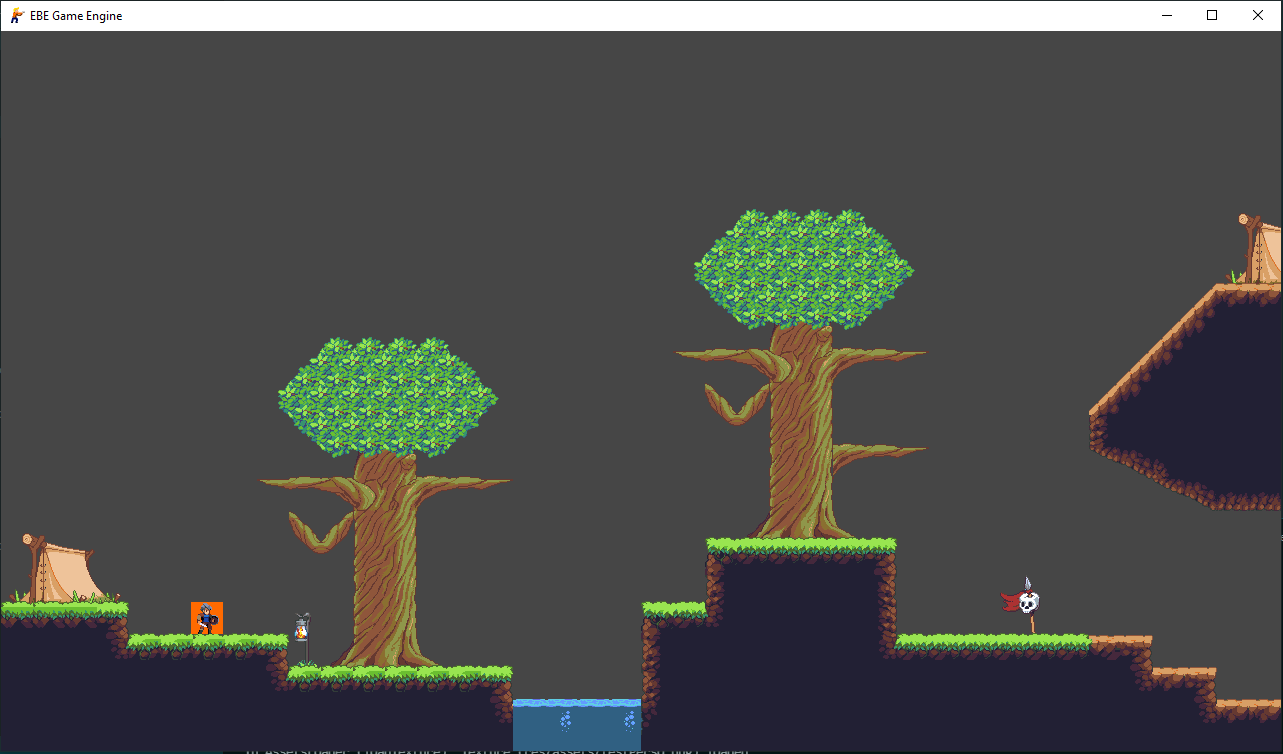
\includegraphics[scale=0.5]{etatJeuActuel.png}
\caption{L'etat du jeu en fin de projet}
\end{figure}
\\[0.5cm]
\indent Nous avons une carte, ainsi qu'un personnage pouvant se d\'eplacer librement sur cette derni\`ere.

\chapter{Analyse des besoins du projet}
Tout d'abord, j'ai entrepris des recherches sur les moteurs de jeu. Lors de ces derni\`eres, j'ai trouv\'e deux principaux mod\`eles de  moteur de jeu :
\begin{itemize}
\item Le mod\`ele bas\'e sur le paradigme de l'orient\'e objet;
\item Le mod\`ele bas\'e sur le paradigme de l'orient\'e donn\'ee, ;
\end{itemize}
\indent J'ai, dans un premier temps, pens\'e \`a choisir le paradigme orient\'e objet, \'etant donn\'e que nous l'avons beaucoup travaill\'e lors de ces derniers semestres. Mais apr\`es r\'eflexions, pour un moteur de jeu, l'orient\'e objet atteint ses limites. Prenons l'exemple simple suivant :
\\[0.2cm]
\begin{figure}[!h]
\centering
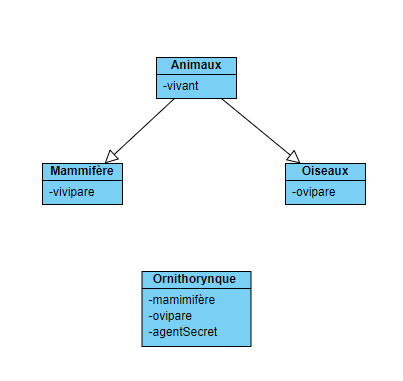
\includegraphics[scale=1]{illustrationOO.png}
\caption{Le patterne orient\'e objet}
\end{figure}
\newpage
~\\[1cm]
\indent Dans cet exemple, nous avons une classe abstraite Animaux, dont h\'eritent deux classes, Mammif\`eres et Oiseaux. Les Mammif\`eres sont vivipares tandis que les Oiseaux sont ovipares. Dans ce cas, quid de l'Ornithorynque, ce mammif\`ere ovipare ? Il est vrai qu'en C++, il y a la possibilit\'e d'h\'eritages multiples, mais cela peut poser d'autres probl\`emes, comme dans l'exemple au dessus, si la classe Oiseaux a un attribut ailes, alors Ornithorynque ne devrait pas h\'eriter d'Oiseaux.
\\
\indent C'est l\`a o\`u le paradigme de l'orient\'e donn\'ee entre en jeu : \\[0.2cm]
\begin{figure}[!h]
\centering
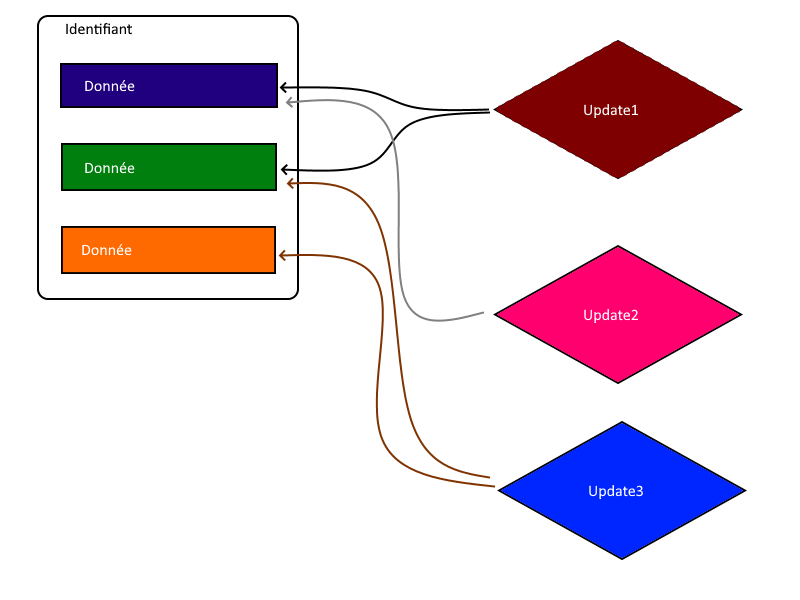
\includegraphics[scale=0.7]{illustrationOD.png}
\caption{Le patterne orient\'e donn\'ee}
\end{figure}
\\[0.2cm]
\indent Dans ce paradigme, nous associons des donn\'ees \`a un identifiant, qui seront manipul\'e par des fonctions en les r\'ecup\'erant selon leur identifiant.
\\
\indent Dans le d\'eveloppement de jeux-vid\'eo, l'utilisation de ce paradigme m\`ene \`a un patterne nomm\'e ECS, pour Entity Component System. Les Entity (entit\'es) sont les identifiants, les Components (composants) sont les donn\'ees, et les Systems (syst\`emes) sont les fonctions. %J'ai d\'ecid\'e d'impl\'ementer l'ECS en C++, et d'utiliser la biblioth\`eque graphique SDL2.

\chapter{Moyens utilis\'es pour la conception du jeu}

\vspace{1cm}
\section{Pour le d\'eveloppement du jeu}
\subsection{Langage C++}
Pour la r\'ealisation du projet, j'ai choisi d'utiliser le langage de programmation C++, car c'est un langage de bas niveau, permettant une gestion assez pouss\'ee de la gestion de la m\'emoire, ce qui est indispensable afin de rendre le jeu utilisable sur le maximum de machines, qu'importe leur puissance. J'ai utilis\'e la biblioth\`eque standard C++17, qui dispose de classes conteneurs tr\`es utiles, comme des tableaux associatifs ou des files, grâce \`a la STL (Standard Template Library).

\subsection{Biblioth\`eque graphique SDL2}
Quant \`a la partie graphique, j'ai choisi d'utiliser la biblioth\`eque SDL2 (Simple Directmedia Layer), \'etant donn\'e que nous l'avons d\'ej\`a manipul\'e au semestre 3 lors du module D\'eveloppement d'Application, et que je l'utilise \'egalement dans certains de mes projets personnels. J'ai \'egalement utilis\'e la d\'ependance SDL\_image, permettant l'utilisation d'images de diff\'erents formats, notamment PNG, l\`a o\`u la biblioth\`eque de base ne permet que l'utilisation du format BMP.
\\
J'ai utilis\'e la version 2.0.16 de la biblioth\`eque, et 2.0.5 pour sa d\'ependance.

\subsection{Biblioth\`eque  d'analyse syntaxique TinyXML}
Finalement, pour une raison que j'aborde dans de la partie suivante, j'ai d\'ecid\'e d'utiliser la biblioth\`eque TinyXML, qui est un parseur (analyseur syntaxique) du format XML. J'ai choisi cette derni\`ere en particulier car elle est de loin la plus simple d'utilisation que j'ai trouv\'e.
\vfill
%\newpage
\section{Pour les ressources graphiques}
\subsection{Itch.io}
%OPP 2017 - Jungle and temple set
%Generic Character Asset v 0.2
N'\'etant pas un fin dessinateur, j'ai d\'ecid\'e d'utiliser des supports visuels libres de droits pr\'e-existants. Pour cela, j'ai cherch\'e sur itch.io, un site web utilis\'e par des cr\'eateurs ind\'ependants pour distribuer leur travaux. Je me suis bien assur\'e que les ressources choisies \'etaient libres de droits avant de les utiliser, puis je les ai arrang\'e pour former un jeu de tuiles, notamment pour le logiciel suivant.
\begin{figure}[!h]
\centering
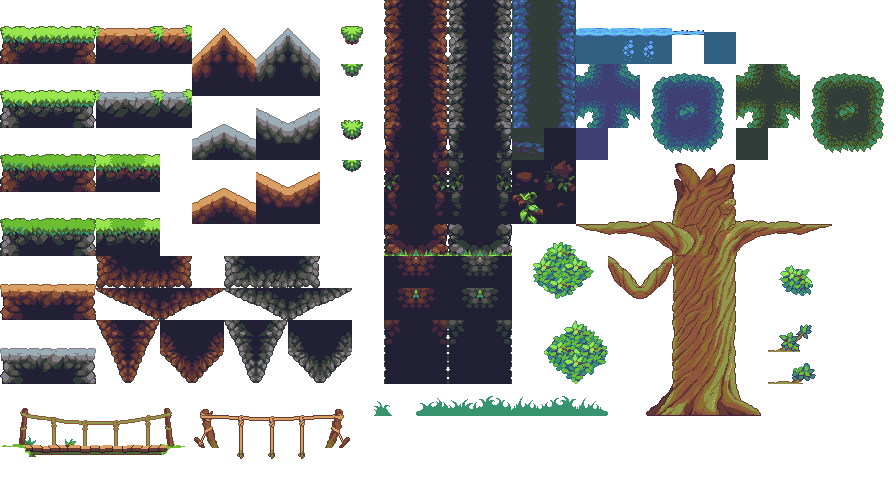
\includegraphics[scale=0.3]{Jungle_terrain.png}
\caption{Le jeu de tuiles form\'e}
\end{figure}

\subsection{Logiciel Tiled Map Editor}
Ce logiciel permet la conception de cartes \`a l'aide de tilesets (jeux de tuiles). Apr\`es conception de la carte, nous obtenons un fichier au format TMX (Tiled's Map Format), d\'eriv\'e du langage XML, justifiant le besoin de la biblioth\`eque TinyXML, contenant les informations du jeu de tuiles ainsi que celles de chaque couches de la carte form\'ee dans le logiciel. J'ai utilis\'e la derni\`ere version de ce logiciel (1.8.0).
\begin{figure}[!h]
\centering
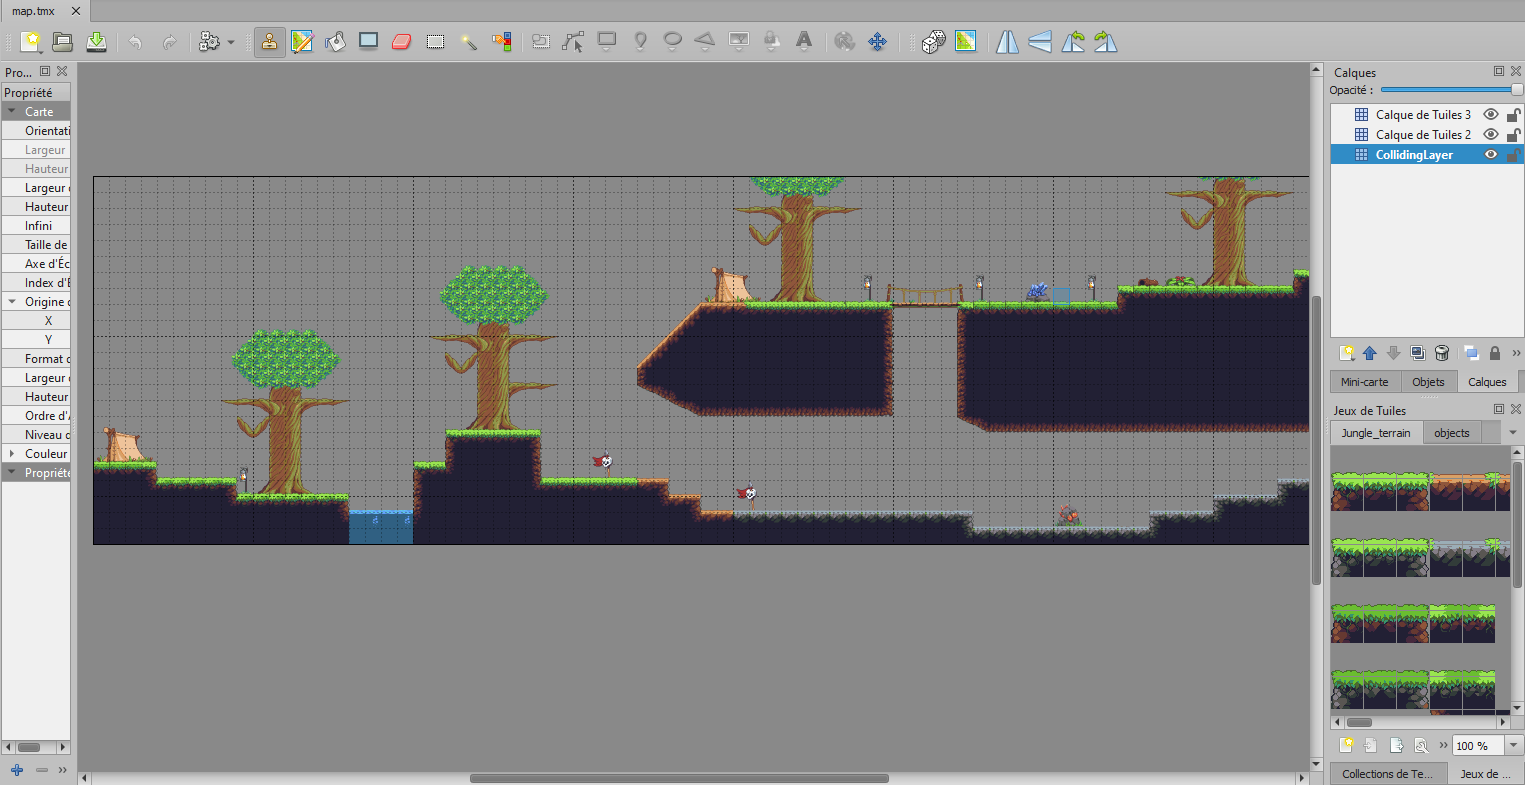
\includegraphics[scale=0.3]{tmxMap.png}
\caption{La carte cr\'e\'ee sur Tiled Map Editor}
\end{figure}
%\\[0.2cm]

\chapter{Analyse des solutions apport\'ees}
\vspace{1cm}
\section{\'Evaluation du temps pr\'evu et du temps r\'eel utilis\'e pour concevoir le projet}
\begin{figure}[!h]
\centering
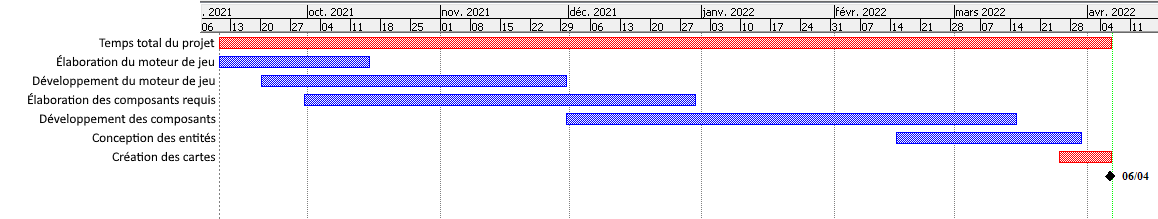
\includegraphics[scale=0.6]{ganttInit_anot.png}
\caption{Temps initialement pr\'evu pour le projet}
\end{figure}
\vspace{0.5cm}
\begin{figure}[!h]
\centering
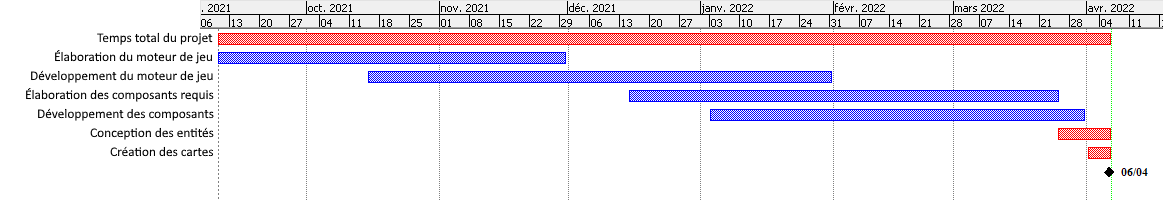
\includegraphics[scale=0.6]{ganttFinal_anot.png}
\caption{Temps r\'eellement pass\'e pour le projet}
\end{figure}
Nous pouvons voir, gr\^ace aux diagrammes de Gantt ci-dessus, que j'ai bien trop sous-estim\'e la conception du moteur de jeu, qui m'a pris cinq mois au lieu des trois que je pr\'evoyais, ce qui m'a pouss\'e \`a pr\'ecipiter la conception des composants. De ce fait, je n'ai pas eu le temps de concevoir ni d'autres entités que le joueur, ni plus d'une carte.

\newpage
%\vspace{1cm}
\section{Analyse et conception de l'ECS}
Afin de concevoir l'Entity Component System, j'ai d\'etermin\'e les besoins :
\begin{itemize}
\item Des entités, qui servent des identifiants, pouvant donc se r\'esumer \`a des entiers;
\item Des composants, contenant des donn\'ees, mais surtout l'entité \`a laquelle ils sont associ\'es;
\item Des tableaux regroupant les composants par type;
\item Un tableau regroupant les tableaux de composants;
\item Les syst\`emes, mettant \`a jour les composants;
\item Des tableaux de bool\'een, pour savoir si un composant est associ\'e \`a une entit\'e;
\item Un tableau regroupant les diff\'erents syst\`emes;
\item Une classe englobant les diff\'erents tableaux afin de centraliser l'ECS.
\end{itemize}
Les entit\'es n'\'etant, comme dit plus haut, que des identifiants, on peut limiter l'entit\'e \`a un entier, d'o\`u le choix de repr\'esenter l'entit\'e comme dessous : 
\begin{figure}[!h]
\centering
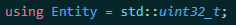
\includegraphics[scale=1]{entity.png}
\caption{D\'efinition du type Entity}
\end{figure}
\par Les composants doivent \^etre s\'epar\'e selon leur type, un composant A ne devant pas \^etre dans le du conteneur du composant B. Pour cela, l'interface des composants utilise un template : le composant h\'eritant de l'interface IComponent doit \^etre du type impl\'ement\'e, expliquant le choix de la d\'efinition de l'interface IComponent comme une classe g\'en\'erique. De plus, la surcharge de l'op\'erateur d'\'egalit\'e permettra de savoir si un composant existe d\'ej\`a pour une entit\'e donn\'ee ou non. Ce qui donne :
\begin{figure}[!h]
\centering
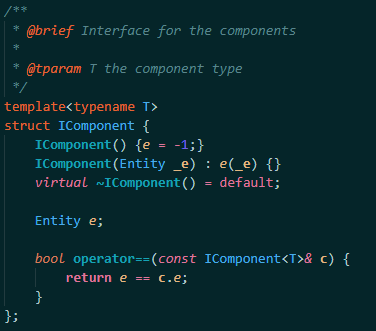
\includegraphics[scale=1]{component.png}
\caption{D\'efinition du type IComponent}
\end{figure}
\newpage
\par Les tableaux de composants sont d\'efinit dans une classe ind\'ependante, mais h\'eritent d'une interface qui oblige l'impl\'ementation d'une fonction \textit{entityDestroyed}, qui assure de supprimer les composants d'une entit\'e d\'etruite, pour \'eviter que, si l'entit\'e est r\'eutilis\'ee, les composants li\'es \`a l'ancienne entit\'e subsistent :
\begin{figure}[!h]
\centering
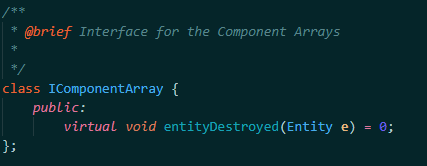
\includegraphics[scale=1]{compArr.png}
\caption{D\'efinition du type IComponentArray}
\end{figure}
\par Le syst\`eme a besoin d'une m\'ethode pour mettre \`a jour les composants, une m\'ethode determinant si une entit\'e peut \^etre mise \`a jour par ce syst\`eme, et un tableau de bool\'een qui d\'etermine quels composants sont requis pour que le syst\`eme mette une entit\'e \`a jour :
\begin{figure}[!h]
\centering
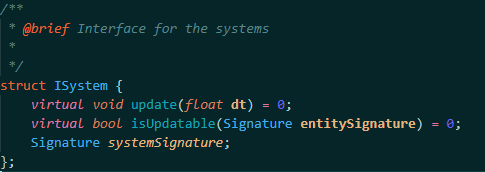
\includegraphics[scale=1]{system.png}
\caption{D\'efinition du type ISystem}
\end{figure}
\par Le type \textit{Signature} est un bitset, un tableau de bits, servant de bool\'een. J'ai \'egalement d\'efini des fonctions attribuant des identifiants aux diff\'erents composants et syst\`emes, pour savoir quel index du bitset est associ\'e \`a quel composant.
\newpage
\begin{figure}[!h]
\centering
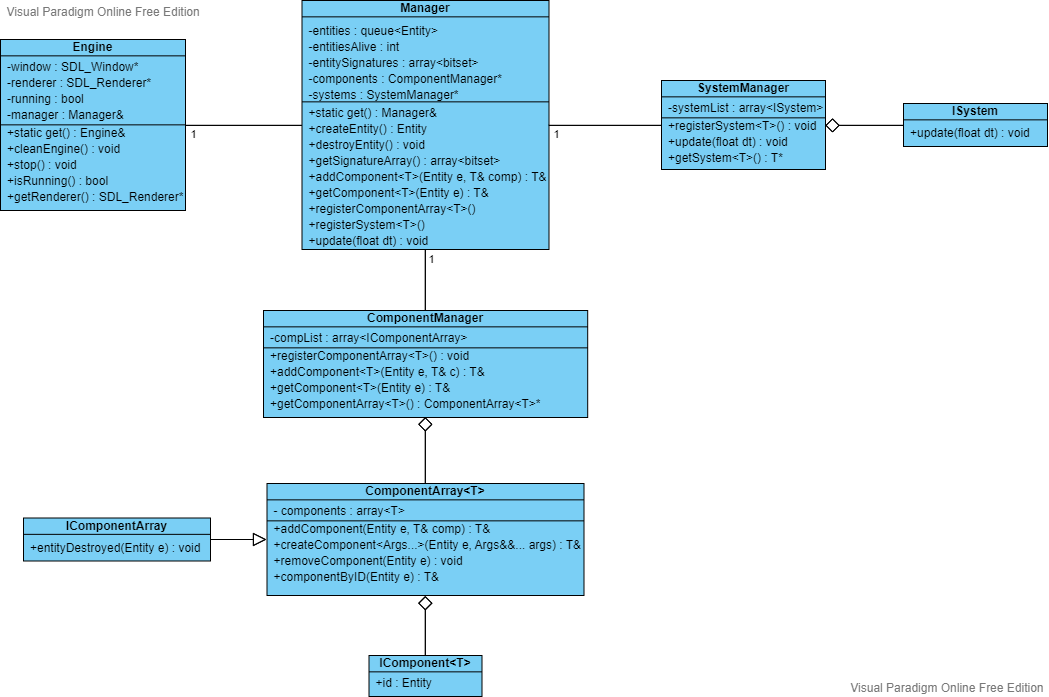
\includegraphics[scale=0.4]{umlECS.png}
\caption{Diagramme UML de l'Entity Component System}
\end{figure}
\par Ci-dessus le diagramme UML de mon Entity Component System. Les classes Manager et Engine sont des objets auto-instanciables, utilisant un patterne similaire au Singleton, mais sans pointeurs. Les templates de \textit{IComponent} et \textit{ComponentArray} sont utilis\'e avec les composants impl\'ementant l'interface \textit{IComponent}.

\section{Analyse des composants}
En pr\'eambule de cette section, je pr\'ecise ce qu'est la structure Vec2, utilis\'ee dans presque tous les composants. Il s'agit d'un vecteur, comportant un x et un y, d\'efinissant par exemple une position dans l'espace. Dans une fen\^etre de la biblioth\`eque SDL2, un Vec2(0,0) correspond au coin haut-gauche.

\noindent
\begin{minipage}{.6\textwidth}
\par Le composant Transform repr\'esente la position d'une entit\'e. Si l'entit\'e a un Sprite (dont on parlera plus loin), le composant Transform d\'etient \'egalement l'\'echelle et la rotation du Sprite. Finalement, si l'entit\'e a un Collider2 et un RigidBody (dont on parlera \'egalement plus loin), Transform contient \'egalement la derni\`ere position s\^ure de l'entit\'e, c'est-\`a-dire la derni\`ere position o\`u l'entit\'e ne traverse pas le sol ou une autre entit\'e.
\end{minipage}
\hfill
\begin{minipage}{.35\textwidth}
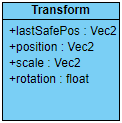
\includegraphics[width=\textwidth]{transform.png}
\end{minipage}
\vspace{0.3cm}
\noindent
\begin{minipage}{.35\textwidth}
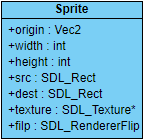
\includegraphics[width=\textwidth]{sprite.png}
\end{minipage}
\hfill
\begin{minipage}{.6\textwidth}
\par Le composant Sprite d\'etient la texture de l'entit\'e. Il contient \'egalement un vecteur repr\'esentant le centre du Sprite, la largeur et la hauteur de la texture, ainsi que l'\'eventuel retournement de la texture (si le personnage court \`a gauche, par exemple, il sera retourn\'e vers la gauche). Finalement, il contient deux rectangles : le rectangle destination, qui repr\'esente la position effective \`a l'\'ecran, et le rectangle source, qui repr\'esente la position du Sprite dans la texture (si le Sprite est anim\'e, par exemple, la position x et y du Sprite changera lors des mises \`a jour).
\end{minipage}
\vspace{0.3cm}
\noindent
\begin{minipage}{.6\textwidth}
\par Le composant Animation d\'etermine si une entit\'e a un Sprite anim\'e ou non. Ce composant d\'etient le nombre de lignes et de colonnes du Sprite anim\'e (la ligne 1 sera, pour les personnages, l'animation d'attente, la deux sera l'animation de course, et la trois aurait \'et\'e l'animation de saut). Il contient aussi la position actuelle de la colonne et de la ligne, ainsi que la vitesse d'animation (le nombre de millisecondes entre chaque changement de colonnes).
\end{minipage}
\hfill
\begin{minipage}{.35\textwidth}
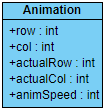
\includegraphics[width=\textwidth]{animation.png}
\end{minipage}
\vspace{0.3cm}
\noindent
\begin{minipage}{.35\textwidth}
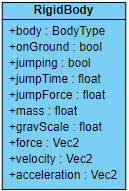
\includegraphics[width=\textwidth]{rigidbody.png}
\end{minipage}
\hfill
\begin{minipage}{.6\textwidth}
Le composant RigidBody repr\'esente le corps physique de l'entit\'e. Il contient plusieurs vecteurs, notamment la force appliqu\'ee \`a l'entit\'e, son acc\'el\'eration et sa v\'elocit\'e. Il y a \'egalement deux bool\'eens, d\'eterminant si le personnage est en train de sauter ou s'il est sur le sol, ainsi que 4 nombres, repr\'esentant la masse du corps, l'\'echelle de gravit\'e appliqu\'ee \`a ce dernier (la gravit\'e est ici un vecteur constant ayant un y \'egal \`a la constante de gravitation terrestre), le temps de saut et la force du saut.
\end{minipage}
\newpage
\noindent
\begin{minipage}{.6\textwidth}
\par Le composant Collider2 repr\'esente la hitbox de l'entit\'e. Il contient le rectangle de la hitbox, ainsi qu'une marge.
\end{minipage}
\hfill
\begin{minipage}{.35\textwidth}
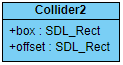
\includegraphics[width=\textwidth]{collider.png}
\end{minipage}
\\[0.5cm]
\par De plus, j'ai cr\'e\'e deux composants sp\'eciaux, le premier est le composant Camera, qui est un composant auto-instanciable repr\'esentant la vue de l'utilisateur, d\'eplacant la carte au gr\'e des d\'eplacements de l'entit\'e du joueur.
\begin{figure}[!h]
\centering
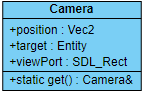
\includegraphics[scale=1.5]{camera.png}
\caption{Composant Camera}
\end{figure}
\\[0.5cm]
\par Le second est le composant Inputs, comportant deux m\'ethodes, \textit{keyUp} et \textit{keyDown}, mettant \`a jour l'unique attribut du composant, un tableau d'entier repr\'esentant l'\'etat du clavier, c'est-\`a-dire quelles touches sont press\'ees ou ne le sont pas.
\begin{figure}[!h]
\centering
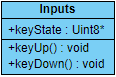
\includegraphics[scale=1.5]{inputs.png}
\caption{Composant Inputs}
\end{figure}
\newpage
\section{Analyse des syst\`emes}
Du c\^ot\'e des syst\`emes, on commence par percevoir les entr\'ees, puis on met \`a jour les composants, avant de les afficher \`a l'\'ecran.
\\
\par Tout d'abord, le syst\`eme d'entr\'ee : la premi\`ere \'etape, c'est de voir quelle entit\'e a les composants Inputs et RigidBody. Ensuite, on r\'ecup\`ere ces composants gr\^ace au gestionnaire central des composants et des syst\`emes. Puis on r\'einitialise la force appliqu\'ee au corps de l'entit\'e. Si l'entit\'e a un composant Animation, on la remet sur l'animation d'attente. On per\c cois apr\`es cela les \'ev\'enements. Finalement, on r\'esout les entr\'ees, gr\^ace aux fonctions d'assistance \textit{isKeyUp} et \textit{isKeyDown}.
\begin{figure}[!h]
\centering
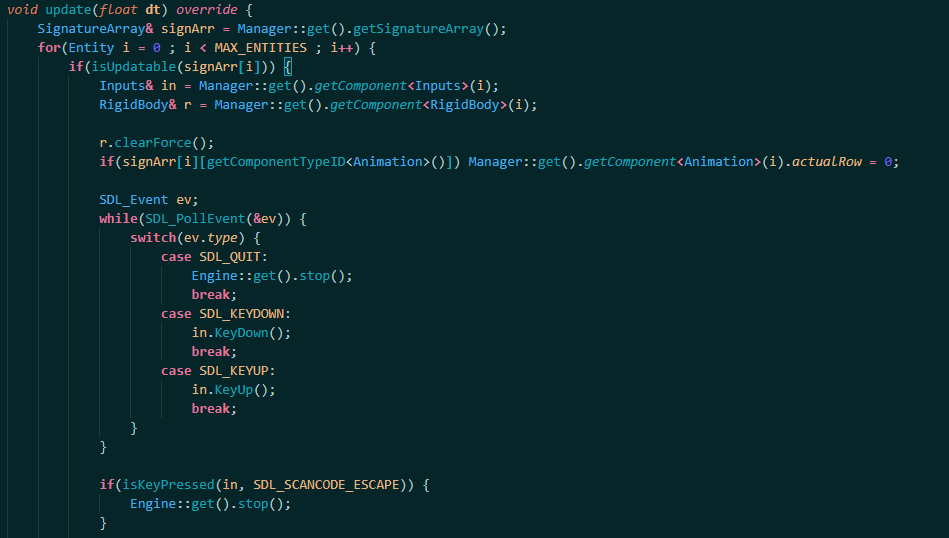
\includegraphics[scale=0.5]{inputsys.png}
\caption{Syst\`eme d'entr\'ee}
\end{figure}
\\[0.2cm]
\begin{figure}[!h]
\centering
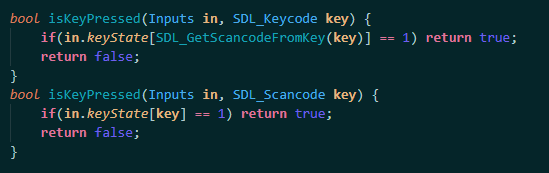
\includegraphics[scale=1]{inputsys2.png}
\caption{Fonctions d'assistance isKeyUp et isKeyDown}
\end{figure}
\newpage
Ensuite, tous les syst\`emes sont bas\'es sur la m\^eme structure : on v\'erifie que l'entit\'e a bien les composants n\'ecessaires, si oui, il le met \`a jour, si non on teste la prochaine entit\'e. Par exemple, voici le syst\`eme de physique :
\begin{figure}[!h]
\centering
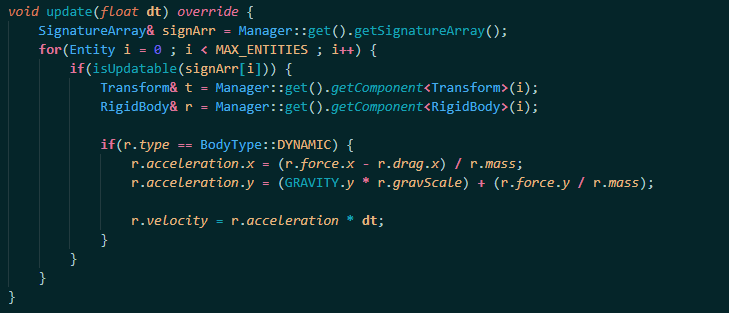
\includegraphics[scale=0.7]{physicsys.png}
\caption{La fonction update de PhysicSystem}
\end{figure}
\\
\par Dans ce syst\`eme, on calcule l'acc\'el\'eration du corps en fonction de la force, qui est mise \`a jour dans le syst\`eme d'entr\'ee, puis la v\'elocit\'e en fonction de l'acc\'el\'eration et du temps syst\`eme. La position, elle, est mise \`a jour dans le syst\`eme de collision, car si elle \'etait mise \`a jour avant la gestion des collision, l'entit\'e pourrait passer au travers de la carte.
\begin{figure}[!h]
\centering
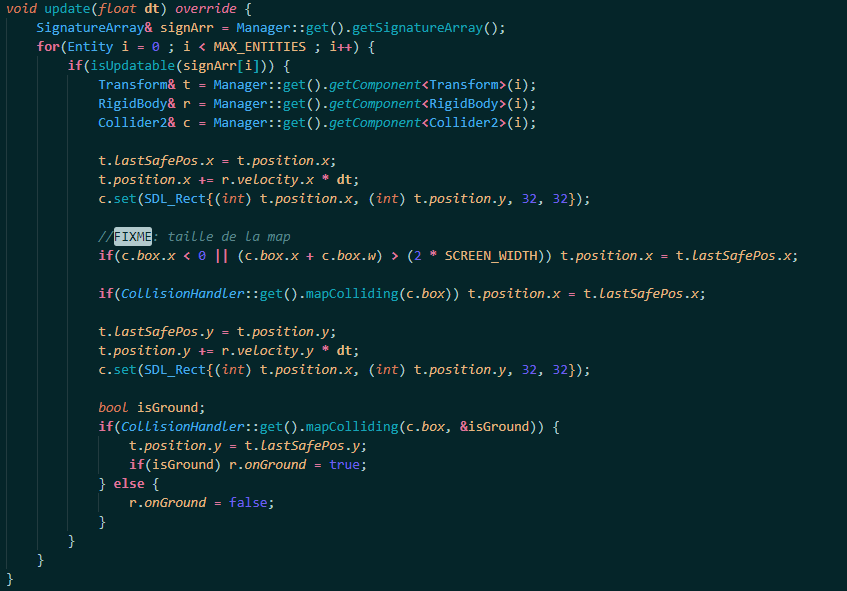
\includegraphics[scale=0.7]{collisionsys.png}
\caption{La fonction update de CollisionSystem}
\end{figure}

\chapter{Conclusion}
Premi\`erement, je dirais que je n'ai pas r\'eussi \`a atteindre les objectifs que je m'\'etais fix\'e. Apr\`es pr\`es de huit mois de travail, je n'ai atteint que deux tiers de l'objectif. J'ai pu conceptualiser un moteur de jeu tr\`es simple, bas\'e sur le patterne de l'Entity Component System, et j'ai pu produire une petite d\'emonstration technique de ce moteur.
\\
\par Cependant, mon objectif n'\'etait pas que le moteur de jeu mais un jeu complet, avec les \'ev\'enements, l'usine \`a entit\'e, nom donn\'e aux fonctions (ou \`a la classe) facilitant la cr\'eation d'entit\'es pr\'ed\'efinies (le joueur, les personnages non-joueurs, les ennemis...). Il me manque de plus les composants permettant de tirer des projectiles, de faire en sorte que les ennemis poursuivent le joueur, ainsi que les d\'eclencheurs, et plusieurs autres cartes.
\\
\par
Je dirais en conclusion de ce rapport que la conception d'un moteur de jeu est bien diff\'erente que celle d'un jeu, et que l'objectif de mon projet aurait d\^u se limiter au moteur de jeu. Malgr\'e cela, gr\^ace \`a ce projet, j'ai appris diff\'erents patternes de d\'eveloppement que nous n'avons pas vu dans notre Licence, ainsi que la syntaxe du C++.

\chapter*{Bibliographie}
\addcontentsline{toc}{chapter}{Bibliographie}
Pour la partie graphique :
\begin{itemize}
\item Ressources du jeu de tuiles : \href{https://openpixelproject.itch.io/opp2017jungle}{OPP 2017 - Jungle and temple set}
\item Ressources du sprite du personnage : \href{https://brullov.itch.io/generic-char-asset}{Generic Character Asset v 0.2}
\end{itemize}
~\\[1cm]
Pour la partie programmation :
\begin{itemize}
\item Recherches sur l'ECS : \href{http://guillaume.belz.free.fr/doku.php?id=ecs}{L'Entity Component System - Qu'est ce que c'est et comment bien s'en servir ? - Guillaume Belz}
\item Recherches sur l'ECS : \href{https://en.wikipedia.org/wiki/Entity_component_system}{Entity Component System - Wikipedia}
\item Recherches sur l'ECS : \href{https://cowboyprogramming.com/2007/01/05/evolve-your-heirachy/}{Evolve your hierarchy - cowboyprogramming}
\item Recherches sur l'ECS : \href{https://www.youtube.com/watch?v=NTWSeQtHZ9M}{Implementation of a component-based entity system in modern C++ - Vittorio Romeo \`a la CppCon 2015}
\item Recherches sur les composants : \href{https://docs.unity3d.com/Manual/Unity2D.html}{Documentation officielle de Unity2D}
\end{itemize}

\end{document}